%%%%%%%%%%%%%%%%%%%% author.tex %%%%%%%%%%%%%%%%%%%%%%%%%%%%%%%%%%%
%
% sample root file for your "contribution" to a contributed volume
%
% Use this file as a template for your own input.
%
%%%%%%%%%%%%%%%% Springer %%%%%%%%%%%%%%%%%%%%%%%%%%%%%%%%%%


% RECOMMENDED %%%%%%%%%%%%%%%%%%%%%%%%%%%%%%%%%%%%%%%%%%%%%%%%%%%
\documentclass[graybox]{svmult}

% choose options for [] as required from the list
% in the Reference Guide

\usepackage{mathptmx}       % selects Times Roman as basic font
\usepackage{helvet}         % selects Helvetica as sans-serif font
\usepackage{courier}        % selects Courier as typewriter font
\usepackage{type1cm}        % activate if the above 3 fonts are
                            % not available on your system
%
\usepackage{makeidx}         % allows index generation
\usepackage{graphicx}        % standard LaTeX graphics tool
                             % when including figure files
\usepackage{multicol}        % used for the two-column index
\usepackage[bottom]{footmisc}% places footnotes at page bottom
\usepackage{subcaption} %% ADDED
%%% Personal packages
%\usepackage[utf8]{inputenc}

% see the list of further useful packages
% in the Reference Guide

\makeindex             % used for the subject index
                       % please use the style svind.ist with
                       % your makeindex program

%%%%%%%%%%%%%%%%%%%%%%%%%%%%%%%%%%%%%%%%%%%%%%%%%%%%%%%%%%%%%%%%%%%%%%%%%%%%%%%%%%%%%%%%%

\begin{document}
\tableofcontents

\title*{non-protein-coding RNAs as regulators of development in tunicates}
% Use \titlerunning{Short Title} for an abbreviated version of
% your contribution title if the original one is too long
\author{Author A and Author B}
% Use \authorrunning{Short Title} for an abbreviated version of
% your contribution title if the original one is too long
\institute{Author Name \at Name, Address of Institute, \email{writeemail@unal.edu.co}
\and   Author Name \at Name, Address of Institute \email{writeemail@com}}
%
% Use the package "url.sty" to avoid
% problems with special characters
% used in your e-mail or web address
%
\maketitle

\abstract*{Each chapter should be preceded by an abstract (10--15 lines long) that summarizes the content. The abstract will appear \textit{online} at \url{www.SpringerLink.com} and be available with unrestricted access. This allows unregistered users to read the abstract as a teaser for the complete chapter. As a general rule the abstracts will not appear in the printed version of your book unless it is the style of your particular book or that of the series to which your book belongs.
Please use the 'starred' version of the new Springer \texttt{abstract} command for typesetting the text of the online abstracts (cf. source file of this chapter template \texttt{abstract}) and include them with the source files of your manuscript. Use the plain \texttt{abstract} command if the abstract is also to appear in the printed version of the book.}

\abstract{Each chapter should be preceded by an abstract (10--15 lines long) that summarizes the content. The abstract will appear \textit{online} at \url{www.SpringerLink.com} and be available with unrestricted access. This allows unregistered users to read the abstract as a teaser for the complete chapter. As a general rule the abstracts will not appear in the printed version of your book unless it is the style of your particular book or that of the series to which your book belongs.\newline\indent
Please use the 'starred' version of the new Springer \texttt{abstract} command for typesetting the text of the online abstracts (cf. source file of this chapter template \texttt{abstract}) and include them with the source files of your manuscript. Use the plain \texttt{abstract} command if the abstract is also to appear in the printed version of the book.}



\section{Introduction}
\label{sec:1}

noncoding RNAs roles in tunicates development date earliest in the 90`s from the works of Swalla \& Jeffry in which RNAs localized in the yellow crescent or myoplasm, a cytoskeletal domain in oocytes of the ascidian \textit{Styela clava} were discovered \cite{Swalla1995}. This  yellow crescent or YC RNA identified to be present throughout embryonic development was the first example involved in envisioning the future of a growing family of ncRNAs that would play important roles in growth and development in tunicates\cite{Swalla1995}.

This asymmetrically distributed ascidian RNAs were part of the set of many other RNAs known as maternally synthesized cytoplasmically localized RNAs, discovered first in oocytes of Xenopus \cite{Bashirullah1998}

\section{miRNA families origin and evolutionary perspective}
\label{sec:2}

\subsection{Origins and Evolution of MicroRNAs}

MicroRNAs (miRNAs) have been described in almost all animals and plants as
well as diverse unicellular eukaryotes. They are important
post-transcriptional regulators of gene expression affecting a sizable
fraction of all mRNAs \cite{Ameres:13}. Mechanistically, miRNAs depends on
the presence of the evolutionarily even older RNA interference pathways
\cite{Cerutti:06, Shabalina:08} that leads to the suppression of
double-stranded RNA molecules in a cell's cytoplasm. 

Throughout animals, canonical miRNAs are the processed through a
well-characterized pathway. The primary precursor transcript (pri-miRNA) is
transcribed by pol-II. While in most cases the pri-miRNA is a long
noncoding RNA, some miRNAs are processed from protein-coding transcripts,
where they are mostly derived from introns \cite{Lin:06}. In the next step,
hairpin-shaped precursors, the pre-miRNAs, are extracted while the RNA is
still residing in the nucleus. These are exported into the cytoplasm
\cite{Lund:04} and then processed further into miRNA/miRNA* duplexes.  In
the final step the single-stranded mature miR or its complement, the miR*,
is incorporated in RISC complex. Sequence complementarity of miR and mRNA
ensures the targeting specificity \cite{Bartel:13}. As as a consequence,
miRNAs share a set of structural characteristics, most importantly the
extremely stable secondary structure of the precursor hairpin and the 2-bp
overhang of miR and miR* generated by Dicer processing. These features make
it possible to reliably identify miRNAs from short RNA-seq data, see e.g.
\cite{Langenberger:10a, Friedlaender:12, Langenberger:13a}.

Most animal microRNAs are among the most highly conserved genetic elements.
The most stringent selection pressure acts on the mature miR sequence. This
is a consequence of the fact that a single miR typically targets a large
number of mRNAs. Mutations in the mature sequence thus simultaneous affect
many interactions, and thus are almost always selected against. In
conjunction with the stringent requirements on the secondary structure, the
entire precursor is under strong stabilizing selection \cite{Price:11},
explaining the observed high levels of sequence conservation. As a
consequence, even evolutionarily distant homologs of miRNAs can be readily
detected despite the short sequence length. Most efficiently,
\texttt{infernal} \cite{Nawrocki:13} is used for this purpose, since it
makes use of both sequence and structure comparison.  The evolution of
miRNAs can thus be traced back in time with high accuracy
\cite{Hertel:06a}. 

Like other gene families, miRNAs form paralogs \cite{Tanzer:04a, Hertel:12a}
and hence often appear as families as homologous genes. This forms the
basis of the \texttt{miRBase} nomenclature \cite{Ambrose:03a}. A series of
investigations into the phylogenetic distribution of miRNA families showed
that miRNAs are infrequently lost at family level and thus serve as
excellent phylogenetic markers
\cite{Sempere:06, Heimberg:08, Heimberg:10, Wheeler:09}, although the massive
restructuring of the miRNA complement of tunicates is an important
exception to this rule \cite{Fu:08}.

The innovation of new miRNA families is an on-going process. Experimental
surveys of the miRNA repertoir thus have reported a large number of very
young and even species-specific miRNAs \cite{Bentwich:05, Berezikov:06}. The
process was studied quantitatively in fruit flies, where innovation rate of
as many as $12$ new miRNA genes per million years has been estimated
\cite{Lu:08}. This is consistent with the fact that stable hairpins are
abundant structural elements in random RNAs, which makes is not only
possible but actually quite likely that miRNA precursors appear by chance
in transcribed genomic regions \cite{Tanzer:04a, CampoPaysaa:11, Marco:13}.
Of course, only a tiny fraction of these fortuitously processed hairpins
have a function and hance are subject to selection, and an even smaller
subset is conserved over long evolutionary time scales. Detailed studies
showed that evolutionarily young miRNA have comparably low expression
levels. Initially, they go through a phase of relatively fast sequence
evolution \cite{Liang:09, Meunier:12}, which slows down as the selective
pressures from a gradual increase in the number of target site increases. A
large, diverse set of targets then protects against miRNA loss
\cite{Lee:07a}. The rate of gain of miRNA families that retained
essentially permanently amounts to only $1$ per several million years. This
number is consistent with divergence of the miRNA complements between
animal phyla.

Many authors have observed that overall the miRNA repertoire has been
expansing throughout animal evolution in a manner that at least roughly
correlates with morphological complexity
\cite{Hertel:06a, Sempere:06, Niwa:07, Prochnik:07, Lee:07a, Heimberg:08, Peterson:09, Berezikov:11}. 
Several bursts of miRNA innovation have been observed
\cite{Hertel:06a, Heimberg:08, Tanzer:10a, Hertel:15a}, most notably at the
root of the placental mammals, the ancestor of ``free-living'' nematodes,
or the radiation of the drosophilids. Massive morphological simplification,
on the other hand, is sometimes associated with a drastic loss of miRNA
families. This has been observed most prominently for tunicates
\cite{Fu:08, Dai:09}.

%\subsection*{MicroRNAs in Tunicates} 

%\TODO{I think we do not really most of the papers below, since much of the
%  relevant material is already subsumed in the summary above.} 
%It was included on 'Validation and detection of miRNA families in Cionas in this decade' and 'The new era to get deep insights into the repertory of miRNA in other urochordates'.

\subsection{miRNA identification and validation}

The first microRNA (miRNA) in tunicates was discovered in the year 2000 from the work of \textit{Pasquinelli et al., 2000} (CITE) when they were studying the temporal regulation of let-7 during development by using samples of small RNAs of a wide range of animal species, in which the ascidian \textit{Ciona intestinalis} was included as well as other vertebrates, hemichordates, mollusc, annelids, arthropod and other bilateral and nonbilateria animals \cite{Pasquinelli2000}. Later on the year 2003 the same team suggested that let-7 RNA may control the late temporal transitions during development across animal phylogeny \cite{Pasquinelli2003} albeit it was not identified on basal metazoans such as cnidarians and poriferans. 

Then after the era of genome sequencing became available, it was launched in 2005 the computational screening of whole-genomes of non-model organism as tunicates. Beginning with the Cionas \textit{C. intestinalis} and \textit{C. savigni} a profile-based strategy was implemented in the ERPIN program \cite{Legendre2005}. On that work were detected a set of new miRNAs candidates considered as \textit{C. intestinalis} specific such as the members of the family miR-9 and miR-79 and as it was expected, other miRNA families were found homologous between both Cionas like the families miR-124;92;98;325;310-313 and let-7. Coincidentally, by the same year a whole-genomic comparative approach in the urochordate lineage was performed on the species \textit{C. intestinalis, C. savignyi} and \textit{O. dioica}. Using a computational screening of structured ncRNAs based upon homology between predicted precursor hairpin structures  $41$ miRNA candidates were detected including let-7 and other six known candidates in \textit{C. intestinalis} \cite{Missal2005}. After all, the same group in 2007 implemented a structure-based clustering approach in \textit{C. intestinalis} predicted $58$ miRNAs, of which only let-7, miR-7, miR-124, and miR-126 coincided with the previously annotated miRNAs \cite{Will2007}. 

Thus far, the primary focus to identify miRNAs into urochordate linage has been mainly toward the use of computational approaches but soon came up the use of new hybrid strategies combining computational and experimental studies to validate candidate families previously detected. For instance the first bona fide record for \textit{C. intestinalis} was registered in mirBase only in its Release 11. Those first miRNAs records were derived from the work published in 2007 by Norden-Krichmar et al., \cite{Norden-Krichmar2007}. The authors searched for conservation with the seed region of the known mature miRNA sequences from miRBase release 2006 on the whole-genomic sequences of \textit{C. intestinalis} and \textit{C. savignyi}. Those miRNAs were aligned locally using the FASTA/ssearch34 program. Only matches of 90\% identity or better were retained. In further steps these authors studied RNA sequences that folds like hairpin structures with the mature miRNA sequence in the stem region including other typical features exhibit in miRNA hairpins. By manual curation of the genomic sequences predicted by the software mfold which folded like hairpin structures, a set of $18$ miRNA molecules were detected which appeared conserved in both Cionas. After all, using  Northern blot analyses in the adult tissue of \textit{C. intestinalis} the authors confirmed expression of  let-7, miR-7, and miR-126, as well as $11$ other conserved miRNA families.

Until 2008, most of the miRNAs annotations were concentrated in Cionas, but new annotation approaches for other species in tunicates were appearing slowly to increase then the repertory of new miRNAs families in urochordates. In this order of ideas, the first repertory of miRNAs based on non-Cionas species was published by Fu et al., in  2008 for the larvacean \textit{O. dioica} \cite{Fu2008}. At that time the authors were studying the temporal-spatial expression patterns of conserved miRNAs in different developmental stages of oocytes, 1-cell zygote, 2-8 cell embryons, blastulas, gastrulas, tadpoles (in different stages) and animals from 1 to 6 days from \textit{O. dioica}. In this research, small RNAs were isolated, amplified by RT-PCR and rapid amplification of cDNA ends (RACE) of the developmental stages, cloned and sequenced. Blast searches using the sequences of cloned small RNA libraries were used to annotate small RNAs as miRNA candidates. In further steps the recovered  genomic flanking sequences each side of those mapped candidates were used as input to predicted secondary structures by mfold v3.1. This step was used to detect candidates that folds like miRNA hairpins and aimed to decrease the set of false positive potential miRNAs in \textit{O. dioica}. Finally, for this set of potential candidates a developmental miRNA array dot blot analyses were performed to detect miRNA expression. With this approach from $3066$ sequenced small RNA clones only for $55$ miRNAs was detected expression. As a conclusion the authors suggested that those candidates were expressed throughout the short life cycle of \textit{O. dioica} showing that some of them were stocked as maternal determinants prior to rapid embryonic development.  Besides the authors identified a set of sex-specific miRNAs that appeared as male/female gonad differentiation which became apparent and was maintained throughout spermatogenesis \cite{Fu2008}. Unexpectedly, the majority of the miRNAs loci in \textit{O. dioica} were located in antisense orientations into the hosted genes in opposite fashion observed in the majority of the known mammalian miRNAs at that time. 

Between the years 2009 and 2015 the majority of the studies of miRNAs in tunicates were focused into the validation of expression of computational predicted miRNAs in Cionas specially focused in \textit{C. intestinalis} as model organism of tunicates or into the test of new computational approaches as miRTRAP, miRDeep2 and miRRim2 which used next-generation sequencing libraries of small RNAs derived from \textit{C. intestinalis} to validate their algorithms. Then by the year 2016 the first comparative homology based search strategy let us to identify the repertory on miRNAs and other ncRNAs in the carpet sea squirt \textit{Didemnum vexillum} with a preliminary comparative analysis of gain and losses of miRNA families on chordates which included the \textit{Cionas}, \textit{O. dioca} and the colonial tunicate \textit{Botryllus schlosseri} \cite{Velandia-Huerto2016}. By the same year, from the preliminary genome sequence assembled for the Southern Ocean salp, \textit{Salpa thompsoni} (Urochordata, Thaliacea) a set of miRNAs families were detected \cite{Jue2016} and in 2017 the prediction of miRNAs families were reported to the species \textit{Halocynthia roretzi}. On the following two sections we will focus on those stages of the fascinated increased screening of the miRNA repertory in tunicates.

\subsubsection{Validation and detection of miRNA families in Cionas in this decade}

At the end of the last decade the application of next generation sequencing technologies to sequence small RNA libraries changed the common way used to detect expression of miRNAs in many organisms including the tunicates. This technology became in one of the most common approaches that supported methods like RT-PCR, microarrays or dot blotting which were previously used to validate miRNA expression in tunicates. In 2009 after preparing small RNA libraries from various developmental stages including unfertilized eggs, early
embryos, late embryos and adults from  \textit{C. intestinalis} was performed high-throughput sequencing of cDNA with an Illumina 1G Genome Analyzer experiments. These sequencing led to document $80$ miRNAs families for  \textit{C. intestinalis}. Unexpectedly, were detected a distinct species of small RNAs processed outside of the miRNA precursors which were termed as moRs or miRNA-offset RNAs \cite{Shi2009}. Later on, after extracting non-coding conserved regions of whole genome alignments between  \textit{C. intestinalis} and \textit{C. savigny} a set of $12$ million sequences were computationally folded using RNAfold and mfold. Then after combining the following criteria: structure/sequence conservation, homology to known miRNAs, and phylogenetic footprinting the authors detected 
a set of $458$ candidate sequences \cite{Keshavan2010}. Then in order to validate those candidate, RT-PCR and PAGE were conducted to design a custom microarray. After screened them for miRNA expression were identifying that $244$ of the $458$ miRNA predictions were represented either in their microarray data or in the Illumina database constructed previously for small RNA derived from \textit{C. intestinalis} by \cite{Shi2009}. Although they failed to predict $39$ previously characterized miRNAs, it was suggested in this work that \textit{C. intestinalis} genome may encode about $300$ miRNA genes. Then to increase the miRNAs collection in \textit{C. intestinalis} a novel computational strategy for the systematic, whole-genome identification of microRNA from high throughput sequencing information was developed in 2010 by \cite{Hendrix2010}. That method, known as miRTRAP, incorporated not only the mechanisms of microRNA biogenesis but also includes additional criteria regarding the prevalence and quality of small RNAs arising from the antisense strand and the neighboring loci. With that approach, nearly $400$ putative microRNAs loci were detected. In short words these strategy relies on the way how the the biochemical machinery processes pre-miRNA hairpins produces short RNA products. This approach is highly depended on the deep of the small RNAs mapped to a given locus and is highlighted by the authors that the approach requires an accurate assignment of small RNA sequences on their relative positions along the hairpin, that is, miR/miR*, moR/moR* and loop \cite{Hendrix2010}. Again a new approach took advantage of importance to detect miRNAs from the high-throughput sequencing of small RNAs available from \cite{Shi2009}. These approach known as  miRDeep2 improved the algorithm of its first version miRDeep \cite{Friedlander2012} and let to identify with an accuracy of $98.6$\% and $99.9$\% canonical and non-canonical miRNAs in different species. These approach reported $313$ known and $127$ novel ones miRNAs in \textit{C. intestinalis}. 
In the same year the program miRRim2 \cite{Terai2012} was applied to the \textit{C. intestinalis} genome, in which some candidates identified from the work of \cite{Hendrix2010} and the several promising candidates were detected. In 2013, \cite{Kusakabe2013} was investigated the expression patterns of the cluster miR-1 and miR-133 in \textit{C. intestinalis} and in \textit{C. savignyi}. RT-PCR amplification of miR-1/133 precursors were performed and PCR products were subcloned and sequenced. Whole-mount in situ hybridization to detect cin-miR-1/miR-133 primary transcript was performed and LNA Northern blotting was conducted on different developmental stages. 

\subsubsection{The new era to get deep insights into the repertory of miRNA in other urochordates}

Since 2016 new approximations has increased our knowledge about new families in other tunicates thanks to the sequence of new urochordate genomes of the species \textit{D. vexillum}, \textit{S. thompsoni} and \textit{H. roretzi} %do not know write here B. schlosseri because no-ncRNAs were reported, only on mtDNA and methodology to validate genes by RNA-seq from different tissues and it was reported on 2013...

(Please summary of our Dvexillum paper \cite{Velandia-Huerto2016} including the first reported preliminary annotation for colonial tunicate \textit{B. schlosseri} beside the one for Dvexillum.)
%%%%ADDED CRISTIAN
For the draft genome sequence from \textit{D. vexillum} an homology-based computational approach was applied \cite{Velandia-Huerto2016}. Blast and HMMer searches were performed with annotated small ncRNAs sequences from metazoans and hidden markov models from RFAM\footnote{\url{http://rfam.xfam.org/}} to obtain the sort of candidates at sequence level. Structural alignments of those sequences were performed by infernal (CITE), using metazoan-specific covariance models to annotate the small ncRNAs collection, which $57$ families and $100$ loci of miRNAs were found. 
%%%%%%%%%%%%
For the preliminary assembled of the genome sequence for the Southern Ocean salp \textit{S. thompsoni} \cite{Jue2016} were small RNA libraries constructed to be sequenced on an Illumina Hiseq 2000. After filtering data sets to 18-24 nt for miRNA and 28-32 nt for piRNA, the reads were aligned to \textit{S. thompsoni} genome and miRNA gene folding predictions were performed using RNAfold. In this initial survey of small RNAs, were revealed the presence of known, conserved miRNAs, as well as novel miRNA genes and mature miRNA signatures for varying developmental stages. Then in 2017, the prediction of $319$ miRNAs candidates in \textit{H. roretzi} were obtained through three complementary methods. The experimental validation suggested that more than half of these candidate miRNAs are expressed during embryogenesis. The expression of some of the predicted miRNAs were validated by RT-PCR using embryonic RNA. In this approach \textit{C. robusta} small RNA-Seq reads derived from \textit{C. robusta} \cite{Shi2009} (previously known as  \textit{C. intestinalis} today reclassified) was used to identify conserved miRNAs in \textit{H. roretzi} \cite{Wang2017} .  

\subsection{miRNA in clusters}

%\begin{figure}[ht!]
%\centering
%\includegraphics[width=\textwidth]{./Images/Cluster_images/let-7_101_128}
%\caption{let-7}.
%\label{fig:dollotree}
%\end{figure}

\begin{figure}[ht!]
\centering
    \begin{subfigure}[t]{1.0\textwidth}
        \centering
        \includegraphics[height=9 cm]{./Images/Cluster_images/let-7_101_128}
        \caption{let-7}
    \end{subfigure}
    \\
    \begin{subfigure}[t]{0.45\textwidth}
        \centering
        \includegraphics[height=1.2 cm]{./Images/Cluster_images/mir-1_119_33}
        \caption{mir-1/mir-133}
     \end{subfigure}
        ~
     \\
    \begin{subfigure}[t]{0.45\textwidth}
        \centering
        \includegraphics[height=1.2 cm]{./Images/Cluster_images/mir-181_105_2502}
        \caption{mir-181}
       \end{subfigure}
        ~
         \begin{subfigure}[t]{0.45\textwidth}
        \centering
        \includegraphics[height=1.2 cm]{./Images/Cluster_images/mir-183_132_240}
        \caption{mir-183}
    \end{subfigure}
    \\
    \begin{subfigure}[t]{0.45\textwidth}
        \centering
        \includegraphics[height=1.2 cm]{./Images/Cluster_images/mir-216_126_467}
        \caption{mir-216/mir-217}
       \end{subfigure}
     \\
    \begin{subfigure}[t]{0.45\textwidth}
        \centering
        \includegraphics[height=1.2 cm]{./Images/Cluster_images/mir-34_11A_435}
        \caption{mir-34}
       \end{subfigure}
        ~
         \begin{subfigure}[t]{0.45\textwidth}
        \centering
        \includegraphics[height=1.2 cm]{./Images/Cluster_images/mir-92_281_4336}
        \caption{mir-92}
    \end{subfigure}
    \\
    \begin{subfigure}[t]{1\textwidth}
        \centering
        \includegraphics[height=1.2 cm]{./Images/Cluster_images/mir-96_138_240}
        \caption{mir-96}
    \end{subfigure}
    \caption{Multiple alignments of miRNA's clusters. \textbf{Prot}: 
Protostomata, \textbf{Brfl}: \textit{B. floridae}, 
\textbf{Oidi}: \textit{O. dioica}, \textbf{Dvex}: \textit{D. vexillum}, 
\textbf{Ciin}: \textit{C. intestinalis}, \textbf{Cisa}: \textit{C. savignyi}, 
\textbf{Ciro}: \textit{C. robusta}, \textbf{Sath}: \textit{S. thompsoni}, 
\textbf{Mata}: \textit{M. oculata}, \textbf{Mlta}: \textit{M. occulta}, 
\textbf{Mlis}: \textit{M. occidentalis}, \textbf{Bosc}: \textit{B. schlosseri}, 
\textbf{Haro}: \textit{H. roretzi}, \textbf{Pema}: \textit{P. marinus}, 
\textbf{Dare}: \textit{D. rerio}, \textbf{Lach}: \textit{L. chalumnae}, 
\textbf{Xetr}: \textit{X. tropicalis} and \textbf{Anca}: \textit{A. 
carolinensis}.}
\end{figure}

\subsubsection{Yanetal2014.pdf}

\cite{Yang2014}
\textit{mir181 is an ancient microRNA (miRNA) gene family that originated in urochordata. Although their functions were subjected to extensive studies in recent years, their evolutionary process remains largely unknown. Here we systematically investigated the homologous genes of the mir-181 family by a sequence similarity search. Representative sequences of the mir-181 gene family were used to reconstruct their evolutionary history. Our results indicated that this family could have derived from multiple duplications, which include two rounds of whole genome duplications and one round of segmental replication. Functional annotation of the target genes of the mir-181 family suggested that this family could participate in some important biological processes including transcriptional and translational regulation, signaling transduction etc. This analysis presented a complex evolutionary dynamics for the origination of a miRNA gene family.}

\subsubsection{Wangetal2017.pdf}
cite{Wang2017}
\textit{Background: miRNAs play essential roles in the modulation of cellular functions via degradation and/or translation
attenuation of target mRNAs. They have been surveyed in a single ascidian genus, Ciona. Recently, an annotated
draft genome sequence for a distantly related ascidian, Halocynthia roretzi, has become available, but miRNAs in
H. roretzi have not been previously studied.
Results: We report the prediction of 319 candidate H. roretzi miRNAs, obtained through three complementary
methods. Experimental validation suggests that more than half of these candidate miRNAs are expressed during
embryogenesis. The majority of predicted H. roretzi miRNAs appear specific to ascidians or tunicates, and only 32
candidates, belonging to 25 families, are widely conserved across metazoans.
Conclusion: Our study presents a comprehensive identification of candidate H. roretzi miRNAs. This resource
will facilitate the study of the mechanisms for miRNA-controlled gene regulatory networks during ascidian
development. Further, our analysis suggests that the majority of Halocynthia miRNAs are specific to ascidian
or tunicates, with only a small number of widely conserved miRNAs. This result is consistent with the general
notion that animal miRNAs are less conserved between taxa than plant ones.}

\subsubsection{deSouzaGomezetal2012.pdf}
\cite{DeSouzaGomes2013}
\textit{MicroRNAs (miRNAs) are small noncoding RNA molecules which are processed into {\~{}}20-24 nt molecules that can regulate the gene expression post-transcriptionally. MiRNA gene clusters have been identified in a range of species, where in miRNAs are often processed from polycistronic transcripts. In this study, a computational approach is used to investigate the extent of evolutionary conservation of the miR-71/2 cluster in animals, and to identify novel miRNAs in the miRNA cluster miR-71/2. The miR-71/2 cluster, consisting of copies of the miR-71 and miR-2 (including miR-13) families, was found to be Protostome-specific. Although, this cluster is highly conserved across the Protostomia, the miR-2 family is completely absent from the Deuterostomia species, while miR-71 is absent from the Vertebrata and Urochordata. The evolutionary conservation and clustering propensity of the miR-71/2 family across the Protostomes could indicate the common functional roles across the member species of the Protostomia.},

\subsubsection{Stadler2007.PDF}
\cite{Will2007}
\textit{The RFAM database defines families of ncRNAs by means of sequence similarities that are sufficient to establish homology. In some cases, such as microRNAs and box H/ACA snoRNAs, functional commonalities define classes of RNAs that are characterized by structural similarities, and typically consist of multiple RNA families. Recent advances in high-throughput transcriptomics and comparative genomics have produced very large sets of putative noncoding RNAs and regulatory RNA signals. For many of them, evidence for stabilizing selection acting on their secondary structures has been derived, and at least approximate models of their structures have been computed. The overwhelming majority of these hypothetical RNAs cannot be assigned to established families or classes. We present here a structure-based clustering approach that is capable of extracting putative RNA classes from genome-wide surveys for structured RNAs. The LocARNA (local alignment of RNA) tool implements a novel variant of the Sankoff algorithm that is sufficiently fast to deal with several thousand candidate sequences. The method is also robust against false positive predictions, i.e., a contamination of the input data with unstructured or nonconserved sequences. We have successfully tested the LocARNA-based clustering approach on the sequences of the RFAM-seed alignments. Furthermore, we have applied it to a previously published set of 3,332 predicted structured elements in the Ciona intestinalis genome (Missal K, Rose D, Stadler PF (2005) Noncoding RNAs in Ciona intestinalis. Bioinformatics 21 (Supplement 2): i77-i78). In addition to recovering, e.g., tRNAs as a structure-based class, the method identifies several RNA families, including microRNA and snoRNA candidates, and suggests several novel classes of ncRNAs for which to date no representative has been experimentally characterized.}

\subsection{miRNA in an perspective evolution}

\subsubsection{Introduction}

\subsubsection{Pignatelli2016.pdf}
\cite{Pignatelli2016}
\textit{Annotation of orthologous and paralogous genes is necessary for many aspects of evolutionary analysis. Methods to infer these homology relationships have traditionally focused on protein-coding genes and evolutionary models used by these methods normally assume the positions in the protein evolve independently. However, as our appreciation for the roles of non-coding RNA genes has increased, consistently annotated sets of orthologous and paralogous ncRNA genes are increasingly needed. At the same time, methods such as PHASE or RAxML have implemented substitution models that consider pairs of sites to enable proper modelling of the loops and other features of RNA secondary structure. Here, we present a comprehensive analysis pipeline for the automatic detection of orthologues and paralogues for ncRNA genes. We focus on gene families represented in Rfam and for which a specific covariance model is provided. For each family ncRNA genes found in all Ensembl species are aligned using Infernal, and several trees are built using different substitution models. In parallel, a genomic alignment that includes the ncRNA genes and their flanking sequence regions is built with PRANK. This alignment is used to create two additional phylogenetic trees using the neighbour-joining (NJ) and maximum-likelihood (ML) methods. The trees arising from both the ncRNA and genomic alignments are merged using TreeBeST, which reconciles them with the species tree in order to identify speciation and duplication events. The final tree is used to infer the orthologues and paralogues following Fitch's definition. We also determine gene gain and loss events for each family using CAFE. All data are accessible through the Ensembl Comparative Genomics ('Compara') API, on our FTP site and are fully integrated in the Ensembl genome browser, where they can be accessed in a user-friendly manner.Database URL: http://www.ensembl.org.}
\subsubsection{Dai2009.pdf}

\cite{Dai2009}
\textit{Cephalochordates, urochordates, and vertebrates comprise the three extant groups of chordates. Although higher morphological and developmental similarity exists between cephalochordates and vertebrates, molecular phylogeny studies have instead suggested that the morphologically simplified urochordates are the closest relatives to vertebrates. MicroRNAs (miRNAs) are regarded as the major factors driving the increase of morphological complexity in early vertebrate evolution, and are extensively characterized in vertebrates and in a few species of urochordates. However, the comprehensive set of miRNAs in the basal chordates, namely the cephalochordates, remains undetermined. Through extensive sequencing of a small RNA library and genomic homology searches, we characterized 100 miRNAs from the cephalochordate amphioxus, Branchiostoma japonicum, and B. floridae. Analysis of the evolutionary history of the cephalochordate miRNAs showed that cephalochordates possess 54 miRNA families homologous to those of vertebrates, which is threefold higher than those shared between urochordates and vertebrates. The miRNA contents demonstrated a clear correlation between the extent of miRNA overlapping and morphological similarity among the three chordate groups, providing a strong evidence of miRNAs being the major genetic factors driving morphological complexity in early chordate evolution.}
\subsubsection{Candini2012.pdf}
\cite{Candiani2012}
\textit{MicroRNAs (miRNAs) are small non-coding RNAs that negatively regulate gene expression and thus control diverse biological processes. The high interest in miRNAs as an important mediator of post-transcriptional gene regulation has led to the discovery of miRNAs in several organisms. The present article outlines and discusses the current status of miRNAs information on the basal chordate amphioxus and the evolution of miRNAs in metazoans.}

\subsubsection{Stadler2006.pdf}
\cite{Hertel2006}
\textit{UNLABELLED: Recently, genome-wide surveys for non-coding RNAs have provided evidence for tens of thousands of previously undescribed evolutionary conserved RNAs with distinctive secondary structures. The annotation of these putative ncRNAs, however, remains a difficult problem. Here we describe an SVM-based approach that, in conjunction with a non-stringent filter for consensus secondary structures, is capable of efficiently recognizing microRNA precursors in multiple sequence alignments. The software was applied to recent genome-wide RNAz surveys of mammals, urochordates, and nematodes. AVAILABILITY: The program RNAmicro is available as source code and can be downloaded from http://www.bioinf.uni-leipzig/Software/RNAmicro.}

\subsubsection{SamGriffit2007.pdf}
\cite{Griffiths-Jones2011}
\textit{MicroRNAs (miRNAs) modulate transcript stability and translation. Functional mature miRNAs are processed from one or both arms of the hairpin precursor. The miR-100/10 family has undergone three independent evolutionary events that have switched the arm from which the functional miRNA is processed. The dominant miR-10 sequences in the insects Drosophila melanogaster and Tribolium castaneum are processed from opposite arms. However, the duplex produced by Dicer cleavage has an identical sequence in fly and beetle. Expression of the Tribolium miR-10 sequence in Drosophila S2 cells recapitulates the native beetle pattern. Thus, arm usage is encoded in the primary miRNA sequence, but outside the mature miRNA duplex. We show that the predicted messenger RNA targets and inferred function of sequences from opposite arms differ significantly. Arm switching is likely to be general, and provides a fundamental mechanism to evolve the function of a miRNA locus and target gene network.},
author = {Griffiths-Jones, Sam and Hui, Jerome H L and Marco, Antonio and Ronshaugen, Matthew}

\subsubsection{Hertel2015.pdf}
\cite{Hertel2015}
\textit{MicroRNAs are important regulatory small RNAs in many eukaryotes. Due to their small size and simple structure, they are readily innovated de novo. Throughout the evolution of animals, the emergence of novel microRNA families traces key morphological innovations. Here, we use a computational approach based on homology search and parsimony-based presence/absence analysis to draw a comprehensive picture of microRNA evolution in 159 animal species. We confirm previous observations regarding bursts of innovations accompanying the three rounds of genome duplications in vertebrate evolution and in the early evolution of placental mammals. With a much better resolution for the invertebrate lineage compared to large-scale studies, we observe additional bursts of innovation, e.g., in Rhabditoidea. More importantly, we see clear evidence that loss of microRNA families is not an uncommon phenomenon. The Enoplea may serve as a second dramatic example beyond the tunicates. The large-scale analysis presented here also highlights several generic technical issues in the analysis of very large gene families that will require further research.}

\subsubsection{Yanetal2014.pdf}


\cite{Yang2014}
\textit{Mir-181 is an ancient microRNA (miRNA) gene family that originated in urochordata. Although their functions were subjected to extensive studies in recent years, their evolutionary process remains largely unknown. Here we systematically investigated the homologous genes of the mir-181 family by a sequence similarity search. Representative sequences of the mir-181 gene family were used to reconstruct their evolutionary history. Our results indicated that this family could have derived from multiple duplications, which include two rounds of whole genome duplications and one round of segmental replication. Functional annotation of the target genes of the mir-181 family suggested that this family could participate in some important biological processes including transcriptional and translational regulation, signaling transduction etc. This analysis presented a complex evolutionary dynamics for the origination of a miRNA gene family. {\textcopyright} 2014 Elsevier Ltd.}

\subsection{To complete the tree of loss and gain of families}

\begin{figure}[ht!]
\centering 
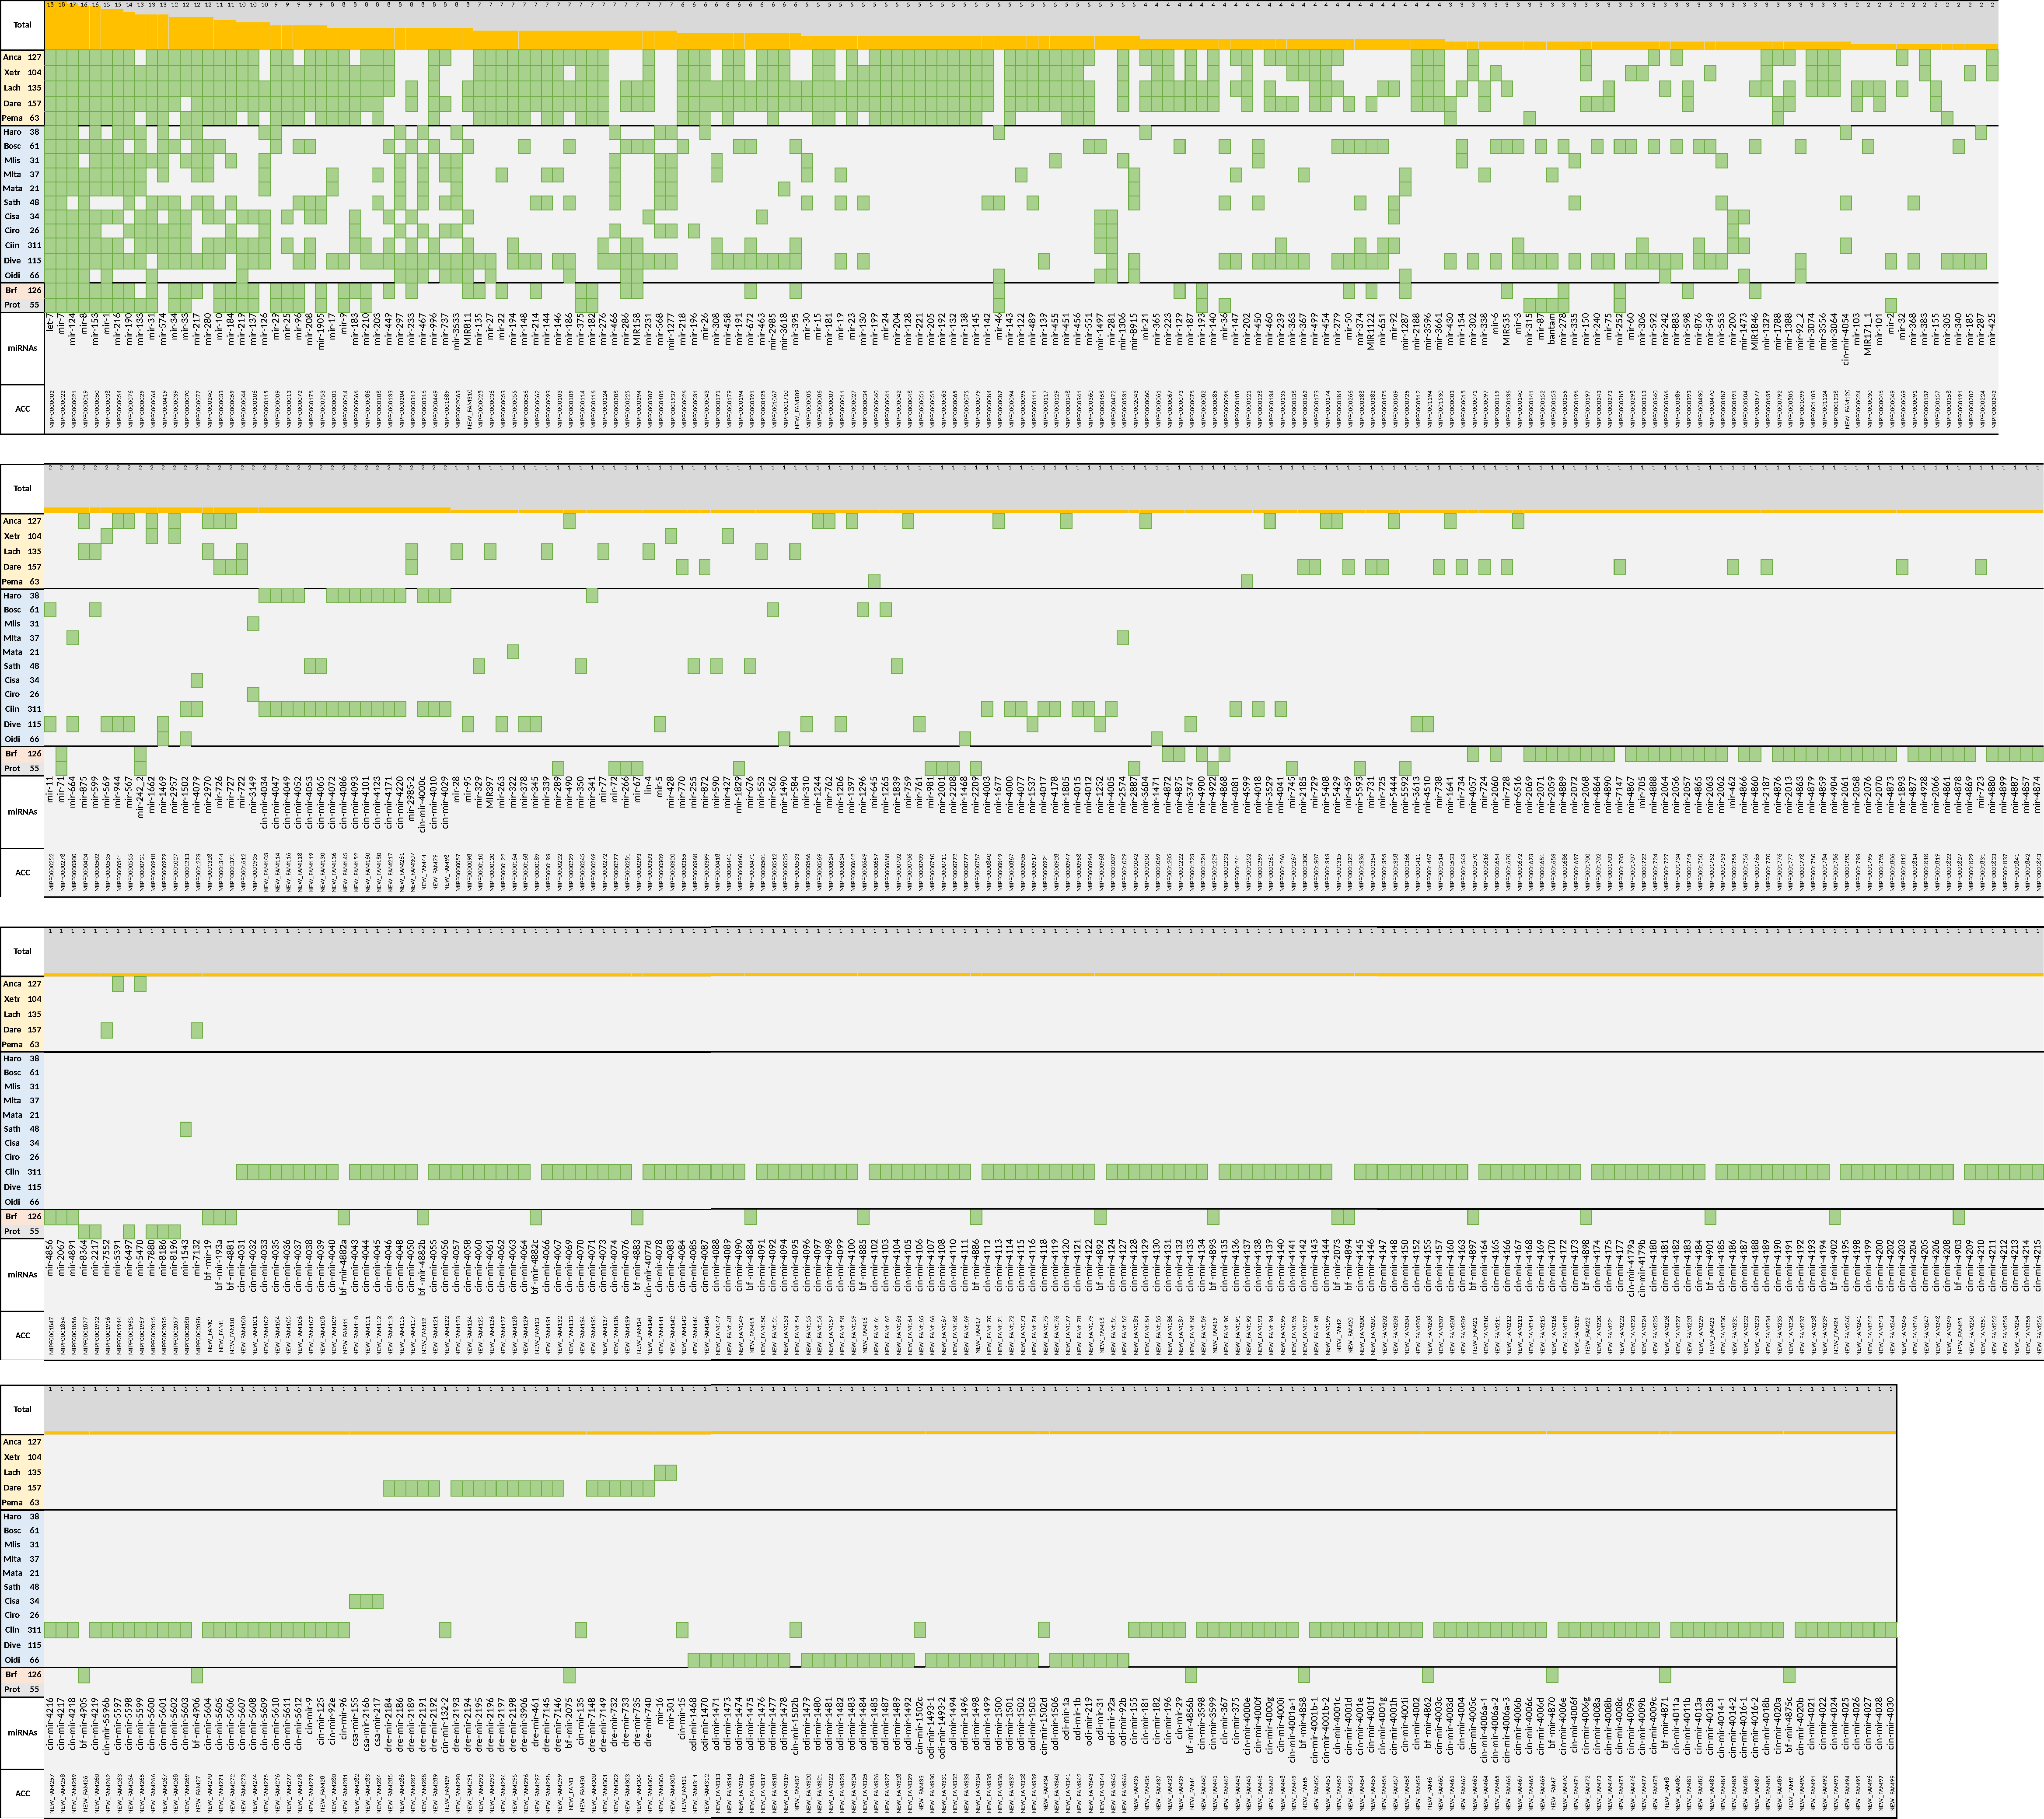
\includegraphics[width=\textwidth, angle=90]{./Images/miRNA_matrix}
\caption{Absence/Presence Matrix of miRNAs families along Bilaterian species. 
\textbf{Prot}: Protostomata, \textbf{Brfl}: \textit{B. floridae}, 
\textbf{Oidi}: \textit{O. dioica}, \textbf{Dvex}: \textit{D. vexillum}, 
\textbf{Ciin}: \textit{C. intestinalis}, \textbf{Cisa}: \textit{C. savignyi}, 
\textbf{Ciro}: \textit{C. robusta}, \textbf{Sath}: \textit{S. thompsoni}, 
\textbf{Mata}: \textit{M. oculata}, \textbf{Mlta}: \textit{M. occulta}, 
\textbf{Mlis}: \textit{M. occidentalis}, \textbf{Bosc}: \textit{B. schlosseri}, 
\textbf{Haro}: \textit{H. roretzi}, \textbf{Pema}: \textit{P. marinus}, 
\textbf{Dare}: \textit{D. rerio}, \textbf{Lach}: \textit{L. chalumnae}, 
\textbf{Xetr}: \textit{X. tropicalis} and \textbf{Anca}: \textit{A. 
carolinensis}. }
\label{fig:matrimirnas}
\end{figure}

Our miRNA families updated with the new two annotated miRNAs Salpa and 
Halocyntia

\begin{figure}[t]
\sidecaption[t]
%\centering
\includegraphics[width=7.5cm]{./Images/last_tree.png}
\caption{Dollo parsymony of miRNAs families distribution in some 
chordates genomes}.
\label{fig:dollotree}
\end{figure}

\begin{figure}[t]
\sidecaption[t]
%\centering
\includegraphics[width=7.4cm]{./Images/cluster_number.pdf} \\ 
\includegraphics[width=7.4cm]{./Images/density.pdf} 
\caption{Analysis of the distribution, size and number's of cluster along chordate species.}
\label{fig:sizeCluster}
\end{figure}

\begin{figure}[t]
\sidecaption[t]
%\centering
\includegraphics[width=7.5cm]{./Images/vennmiRNAs}
\caption{Comparsion between miRNAs families along Bilaterian species. Same 
labels from Figure \ref{fig:matrimirnas} were used. In this case 
\textsl{vertebrates} group the following species: \textbf{Pema}: \textit{P. 
marinus}, \textbf{Dare}: \textit{D. rerio}, \textbf{Lach}: \textit{L. 
chalumnae}, \textbf{Xetr}: \textit{X. tropicalis} and \textbf{Anca}: \textit{A. 
carolinensis}}
\label{fig:vennDiagram}
\end{figure}

\cite{Velandia-Huerto2016} \textit{A comparative analysis of miRNAs families in 
tunicates is summarized in Fig. 5 c and d. We find several patterns of 
recognizable trends as we analyze the conservation, loss and gain of miRNA 
families in tunicates compared to selected bilaterians. For instance, based in 
our analysis of conserved miRNA families across the bilaterians, we estimate 
that ancestor of the Bilateria likely contained approximately 33 miRNA families. 
In contrast, the ancestor of the Chordata presumably contained members of 37 
miRNA families. In the cephalochordate B. floridae, we find the occurrence of a 
unique repertoire of 82 miRNA families that evolved as a consequence of many 
gains (+50), but also some losses (−5) [8]. In the ancestor of Olfactores we 
presume the presence of 72 miRNA families, of which tunicates did not show 
losses, with the notable exception of O. dioica that has undergone substantial 
losses (−60). Within the ascidians, only B. schlosseri and C. savignyi show 
dramatic losses of miRNA families, −32 and −17 respectively. D. vexillum has 
lost 8 miRNA families. D. vexillum shows 16 families that are absent in other 
tunicates i.e. mir-430, mir-9, mir-130, mir-190, mir-139, mir-460, mir-315, 
mir-305, mir-458, mir-185, mir-233, mir-569, mir-944, mir-567, mir-2985 and 
mir-4068 (Fig. 5d). Comparisons of the miRNAs repertoires between the colonial 
tunicates (D. vexillum and B. schlosseri) on the one hand, and solitary 
tunicates (O. dioica, C. intestinalis and C. savignyi) on the other hand, show 
10 microRNA families, i.e. mir-133, mir-186, mir-6, mir-279, mir-340, mir-11, 
mir-60, mir-592, mir-883 and mir-549 that are specific to colonial tunicates, 
while only 2 families, i.e. mir-31 and mir-1473, are specific to olitary 
tunicates. It is worthwhile exploring how colonial specific miRNAs may have been 
co-opted in ascidians to function in somatic stem cell function, regeneration, 
budding, or other asexual developmental processes, as miRNAs are know to be 
important players in stem cell function, and developmental processes of 
differentiation in vertebrates}

\subsubsection{Jueetal2016.pdf}
\cite{Jue2016}
\textit{A preliminary genome sequence has been assembled for the Southern Ocean salp, Salpa thompsoni (Urochordata, Thaliacea). Despite the ecological importance of this species in Antarctic pelagic food webs and its potential role as an indicator of changing Southern Ocean ecosystems in response to climate change, no genomic resources are available for S. thompsoni or any closely-related urochordate species. Using a multiple-platform, multiple-individual approach, we have produced a 318,767,936 bp genome sequence, covering more than 50{\%} of the estimated 602 MB (±173 MB) genome size for S. thompsoni Using a non-redundant set of predicted proteins, more than 50{\%} (16,823) of sequences showed significant homology to known proteins and {\~{}}38{\%} (12,151) of the total protein predictions were associated with Gene Ontology functional information. We have generated 109,958 SNP variant and 9,782 indel predictions for this species, serving as a resource for future phylogenomic and population genetic studies. Comparing the salp genome to available assemblies for four other urochordates, Botryllus schlosseri, Ciona intestinalis, Ciona savignyi and Oikopleura dioica, we found that S. thompsoni shares the previously-estimated rapid rates of evolution for these species. High mutation rates are thus independent of genome size, suggesting that rates of evolution {\textgreater}1.5 times that observed for vertebrates are a broad taxonomic characteristic of urochordates. Tests for positive selection implemented in PAML revealed a small number of genes with sites undergoing rapid evolution, including genes involved in ribosome biogenesis and metabolic and immune process that may be reflective of both adaptation to polar, planktonic environments as well as the complex life history of the salps. Finally, we performed an initial survey of small RNAs, revealing the presence of known, conserved miRNAs, as well as novel miRNA genes; unique piRNAs; and mature miRNA signatures for varying developmental stages. Collectively, these resources provide a genomic foundation supporting S. thompsoni as a model species for further examination of the exceptional rates and patterns of genomic evolution shown by urochordates. Additionally, genomic data will allow for the development of molecular indicators of key life history events and processes and afford new understandings and predictions of impacts of climate change on this key species of Antarctic pelagic ecosystems.}


\subsubsection{Wangetal2017.pdf}
\cite{Wang2017}
\textit{Background: miRNAs play essential roles in the modulation of cellular functions via degradation and/or translation
attenuation of target mRNAs. They have been surveyed in a single ascidian genus, Ciona. Recently, an annotated
draft genome sequence for a distantly related ascidian, Halocynthia roretzi, has become available, but miRNAs in
H. roretzi have not been previously studied.
Results: We report the prediction of 319 candidate H. roretzi miRNAs, obtained through three complementary
methods. Experimental validation suggests that more than half of these candidate miRNAs are expressed during
embryogenesis. The majority of predicted H. roretzi miRNAs appear specific to ascidians or tunicates, and only 32
candidates, belonging to 25 families, are widely conserved across metazoans.
Conclusion: Our study presents a comprehensive identification of candidate H. roretzi miRNAs. This resource
will facilitate the study of the mechanisms for miRNA-controlled gene regulatory networks during ascidian
development. Further, our analysis suggests that the majority of Halocynthia miRNAs are specific to ascidian
or tunicates, with only a small number of widely conserved miRNAs. This result is consistent with the general
notion that animal miRNAs are less conserved between taxa than plant ones.}

\section{miRNAs and its rol in development}
\label{sec:3}

\subsection{miRNAs discovery and development}
%F
\subsubsection{Bartel2004.pdf}

\cite{Bartel2004}
\textit{MicroRNAs (miRNAs) are endogenous $22$ nt RNAs that can play important regulatory roles in animals and plants by targeting mRNAs for cleavage or translational repression. Although they escaped notice until relatively recently, miRNAs comprise one of the more abundant classes of gene regulatory molecules in multicellular organisms and likely influence the output of many protein-coding genes.}
\subsubsection{Lee1993.pdf}

\cite{Lee1993}
\textit{diverse postembryonic developmental events in C.
elegans. /in-4 acts by negatively regulating the level of
LIN-14 protein, creating a temporal decrease in LIN-14
protein starting in the first larval stage (Ll). We have
cloned the C. elegans lin-4 locus by chromosomal
walking and transformation rescue. We used the C.
elegans clone to isolate the gene from three other
Caenorhabditis species; all four Caenorhabditis clones
functionally rescue the h-4 null allele of C. elegans.
Comparison of the /in-4 genomic sequence from these
four species and site-directed mutagenesis of potential
open reading frames indicated that /in-d does not
encode a protein. Two small /in-4 transcripts of approximately
22 and 61 nt were identified in C. elegans and
found to contain sequences complementary to a repeated
sequence element in the 3'untranslated region
(UTR) of lin-74 mRNA, suggesting that /in-4 regulates
h-74 tr}


\subsection{miRNAs perspective evolution in development}
%F
\subsubsection{holland2014.pdf}
\cite{Holland2015} \textit{
Morphological comparisons among extant animals have long been used to infer 
their long-extinct ancestors for which the fossil record is poor or 
non-existent. For evolution of the vertebrates, the comparison has typically 
involved amphioxus and vertebrates. Both groups are evolving relatively slowly, 
and their genomes share a high level of synteny. Both vertebrates and amphioxus 
have regulative development in which cell fates become fixed only gradually 
during embryogenesis. Thus, their development fits a modified hourglass model in 
which constraints are greatest at the phylotypic stage (i.e., the late 
neurula/early larva), but are somewhat greater on earlier development than on 
later development. In contrast, the third group of chordates, the tunicates, 
which are sister group to vertebrates, are evolving rapidly. Constraints on 
evolution of tunicate genomes are relaxed, and they have discarded key 
developmental genes and organized much of their coding sequences into operons, 
which are transcribed as a single mRNA that undergoes trans-splicing. This 
contrasts with vertebrates and amphioxus, whose genomes are not organized into 
operons. Concomitantly, tunicates have switched to determinant development with 
very early fixation of cell fates. Thus, tunicate development more closely fits 
a progressive divergence model (shaped more like a wine glass than an hourglass) 
in which the constraints on the zygote and very early development are greatest. 
This model can help explain why tunicate body plans are so very diverse. The 
relaxed constraints on development after early cleavage stages are correlated 
with relaxed constraints on genome evolution. The question remains: which came 
first?}
\subsubsection{Sun2013.pdf}

\cite{Sun2013}
\textit{MicroRNAs (miRNAs) are {\~{}}22 nt RNAs that coordinate vast regulatory 
networks in animals and thereby influence myriad processes. This Review examines 
evidence that miRNAs have continuous roles in adults in ways that are separable 
from developmental control. Adult-specific activities for miRNAs have been 
described in various stem cell populations, in the context of neural function 
and cardiovascular biology, in metabolism and ageing, and during cancer. In 
addition to reviewing recent results, we also discuss methods for studying miRNA 
activities specifically in adults and evaluate their relative strengths and 
weaknesses. A fuller understanding of continuous functions of miRNAs in adults 
has bearing on efforts and opportunities to manipulate miRNAs for therapeutic 
purposes.}
\subsubsection{Kloosterman2006.pdf}

\cite{Kloosterman2006}
\textit{MicroRNAs (miRNAs) control gene expression by translational inhibition 
and destabilization of mRNAs. While hundreds of miRNAs have been found, only??a 
few have been studied in detail. miRNAs have been implicated in tissue 
morphogenesis, cellular processes like apoptosis, and major signaling pathways. 
Emerging evidence suggests a direct link between miRNAs and disease, and miRNA 
expression signatures are associated with various types of cancer. In addition, 
the gain and loss of miRNA target sites appears to be causal to some genetic 
disorders. Here, we discuss the current literature on the role of miRNAs in 
animal development and disease. ?? 2006 Elsevier Inc. All rights reserved.}

\subsubsection{Iyengar2014.pdf}

\cite{Iyengar2014}
\textit{The human brain is one of the most complex biological systems, and the 
cognitive abilities have greatly expanded compared to invertebrates without much 
expansion in the number of protein coding genes. This suggests that gene 
regulation plays a very important role in the development and function of 
nervous system, by acting at multiple levels such as transcription and 
translation. In this article we discuss the regulatory roles of three classes of 
non-protein coding RNAs (ncRNAs)-microRNAs (miRNAs), piwi-interacting RNA 
(piRNAs) and long-non-coding RNA (lncRNA), in the process of neurogenesis and 
nervous function including control of synaptic plasticity and potential roles in 
neurodegenerative diseases. miRNAs are involved in diverse processes including 
neurogenesis where they channelize the cellular physiology toward neuronal 
differentiation. miRNAs can also indirectly influence neurogenesis by regulating 
the proliferation and self renewal of neural stem cells and are dysregulated in 
several neurodegenerative diseases. miRNAs are also known to regulate synaptic 
plasticity and are usually found to be co-expressed with their targets. The 
dynamics of gene regulation is thus dependent on the local architecture of the 
gene regulatory network (GRN) around the miRNA and its targets. piRNAs had been 
classically known to regulate transposons in the germ cells. However, piRNAs 
have been, recently, found to be expressed in the brain and possibly function by 
imparting epigenetic changes by DNA methylation. piRNAs are known to be 
maternally inherited and we assume that they may play a role in early 
development. We also explore the possible function of piRNAs in regulating the 
expansion of transposons in the brain. Brain is known to express several lncRNA 
but functional roles in brain development are attributed to a few lncRNA while 
functions of most of the them remain unknown. We review the roles of some known 
lncRNA and explore the other possible functions of lncRNAs including their 
interaction with miRNAs.}

\subsection{Specific examples} 
\subsubsection{Chenetal2014.PDF}
\cite{Chen2014}
\textit{Notch-Delta signaling is a fundamental cell-cell communication mechanism 
that governs the differentiation of many cell types. Most existing mathematical 
models of Notch-Delta signaling are based on a feedback loop between Notch and 
Delta leading to lateral inhibition of neighboring cells. These models result in 
a checkerboard spatial pattern whereby adjacent cells express opposing levels of 
Notch and Delta, leading to alternate cell fates. However, a growing body of 
biological evidence suggests that Notch-Delta signaling produces other patterns 
that are not checkerboard, and therefore a new model is needed. Here, we present 
an expanded Notch-Delta model that builds upon previous models, adding a local 
Notch activity gradient, which affects long-range patterning, and the activity 
of a regulatory microRNA. This model is motivated by our experiments in the 
ascidian Ciona intestinalis showing that the peripheral sensory neurons, whose 
specification is in part regulated by the coordinate activity of Notch-Delta 
signaling and the microRNA miR-124, exhibit a sparse spatial pattern whereby 
consecutive neurons may be spaced over a dozen cells apart. We perform rigorous 
stability and bifurcation analyses, and demonstrate that our model is able to 
accurately explain and reproduce the neuronal pattern in Ciona. Using Monte 
Carlo simulations of our model along with miR-124 transgene over-expression 
assays, we demonstrate that the activity of miR-124 can be incorporated into the 
Notch decay rate parameter of our model. Finally, we motivate the general 
applicability of our model to Notch-Delta signaling in other animals by 
providing evidence that microRNAs regulate Notch-Delta signaling in analogous 
cell types in other organisms, and by discussing evidence in other organisms of 
sparse spatial patterns in tissues where Notch-Delta signaling is active.}

\subsubsection{Fuetal2008.pdf}

\cite{Fu2008}
\textit{Recent studies reveal correlation between microRNA (miRNA) innovation 
and increased developmental complexity. This is exemplified by dramatic 
expansion of the miRNA inventory in vertebrates, a lineage where genome 
duplication has played a significant evolutionary role. Urochordates, the 
closest extant group to the vertebrates, exhibit an opposite trend to genome and 
morphological simplification. We show that the urochordate, larvacean, 
Oikopleura dioica, possesses the requisite miRNA biogenic machinery. The miRNAs 
isolated by small RNA cloning were expressed throughout the short life cycle, a 
number of which were stocked as maternal determinants prior to rapid embryonic 
development. We identify sex-specific miRNAs that appeared as male/female gonad 
differentiation became apparent and were maintained throughout spermatogenesis. 
Whereas 80{\%} of mammalian miRNAs are hosted in introns of protein-coding 
genes, the majority of O. dioica miRNA loci were located in antisense 
orientations to such genes. Including sister group ascidians in analysis of the 
urochordate miRNA repertoire, we find that 11 highly conserved bilaterian miRNA 
families have been lost or derived to the point they are not recognizable in 
urochordates and a further 4 of these families are absent in larvaceans. 
Subsequent to this loss/derivation, at least 29 novel miRNA families have been 
acquired in larvaceans. This suggests a profound reorganization of the miRNA 
repertoire integral to evolution in the urochordate lineage.}

\subsubsection{Hendrixetal2010.pdf}
\cite{Hendrix2010}
\textit{MicroRNAs (miRs) have been broadly implicated in animal development and 
disease. We developed a novel computational strategy for the systematic, 
whole-genome identification of miRs from high throughput sequencing information. 
This method, miRTRAP, incorporates the mechanisms of miR biogenesis and includes 
additional criteria regarding the prevalence and quality of small RNAs arising 
from the antisense strand and neighboring loci. This program was applied to the 
simple chordate Ciona intestinalis and identified nearly 400 putative miR loci.}

\subsubsection{Kusakabeetal2013.pdf}
\cite{Kusakabe2013}
\textit{Muscle-specific miR-1/206 and miR-133 families have been suggested to 
play fundamental roles in skeletal and cardiac myogenesis in vertebrates. To 
gain insights into the relationships between the divergence of these miRs and 
muscular tissue types, we investigated the expression patterns of miR-1 and 
miR-133 in two ascidian Ciona species and compared their genomic structures with 
those of other chordates. We found that Ciona intestinalis and Ciona savignyi 
each possess a single copy of the miR-1/miR-133 cluster, which is only 350 
nucleotide long. During embryogenesis, Ciona miR-1 and miR-133 are generated as 
a single continuous primary transcript accumulated in the nuclei of the tail 
muscle cells, starting at the gastrula stage. In adults, mature miR-133 and 
miR-1 are differentially expressed in the heart and body wall muscle. Expression 
of the reporter gene linked to the 850-bp upstream region of the predicted 
transcription start site confirmed that this region drives the muscle-specific 
expression of the primary transcript of miR-1/miR-133. In many deuterostome 
lineages, including that of Ciona, the miR-1/133 cluster is located in the same 
intron of the mind bomb (mib) gene in reverse orientation. Our results suggest 
that the origin of genomic organization and muscle-specific regulation of 
miR-1/133 can be traced back to the ancestor of chordates. Duplication of this 
miR cluster might have led to the remarkable elaboration in the morphology and 
function of skeletal muscles in the vertebrate lineage. {\textcopyright} 2012 
Elsevier B.V. All rights reserved.}

\subsubsection{Pasquinellietal2000.pdf}

\cite{Pasquinelli2000}
\textit{Two small RNAs regulate the timing of Caenorhabditis elegans 
development. Transition from the first to the second larval stage fates requires 
the 22-nucleotide lin-4 RNA, and transition from late larval to adult cell fates 
requires the 21-nucleotide let-7 RNA. The lin-4 and let-7 RNA genes are not 
homologous to each other, but are each complementary to sequences in the 3' 
untranslated regions of a set of protein-coding target genes that are normally 
negatively regulated by the RNAs. Here we have detected let-7 RNAs of 
approximately 21 nucleotides in samples from a wide range of animal species, 
including vertebrate, ascidian, hemichordate, mollusc, annelid and arthropod, 
but not in RNAs from several cnidarian and poriferan species, Saccharomyces 
cerevisiae, Escherichia coli or Arabidopsis. We did not detect lin-4 RNA in 
these species. We found that let-7 temporal regulation is also conserved: let-7 
RNA expression is first detected at late larval stages in C. elegans and 
Drosophila, at 48 hours after fertilization in zebrafish, and in adult stages of 
annelids and molluscs. The let-7 regulatory RNA may control late temporal 
transitions during development across animal phylogeny.}

\subsubsection{Tangetal2013.pdf}
\textit{JoyceTang2013}
\textit{The formation of the sensory organs and cells that make up the 
peripheral nervous system (PNS) relies on the activity of transcription factors 
encoded by proneural genes (PNGs). Although PNGs have been identified in the 
nervous systems of both vertebrates and invertebrates, the complexity of their 
interactions has complicated efforts to understand their function in the context 
of their underlying regulatory networks. To gain insight into the regulatory 
network of PNG activity in chordates, we investigated the roles played by PNG 
homologs in regulating PNS development of the invertebrate chordate Ciona 
intestinalis. We discovered that in Ciona, MyT1, Pou4, Atonal, and NeuroD-like 
are expressed in a sequential regulatory cascade in the developing epidermal 
sensory neurons (ESNs) of the PNS and act downstream of Notch signaling, which 
negatively regulates these genes and the number of ESNs along the tail midlines. 
Transgenic embryos mis-expressing any of these proneural genes in the epidermis 
produced ectopic midline ESNs. In transgenic embryos mis-expressing Pou4, and 
MyT1 to a lesser extent, numerous ESNs were produced outside of the embryonic 
midlines. In addition we found that the microRNA miR-124, which inhibits Notch 
signaling in ESNs, is activated downstream of all the proneural factors we 
tested, suggesting that these genes operate collectively in a regulatory 
network. Interestingly, these factors are encoded by the same genes that have 
recently been demonstrated to convert fibroblasts into neurons. Our findings 
suggest the ascidian PNS can serve as an in vivo model to study the underlying 
regulatory mechanisms that enable the conversion of cells into sensory neurons. 
?? 2013 Elsevier Inc.}

\subsubsection{Spina2017.pdf}

\cite{Spina2017}
\textit{Here we present a parallel study of mRNA and microRNA expression during 
oral siphon (OS) regeneration in Ciona robusta, and the derived network of their 
interactions. In the process of identifying 248 mRNAs and 15 microRNAs as 
differentially expressed (DE), we also identified 57 novel microRNAs, several of 
which are among the most highly DE. Analysis of functional categories identified 
enriched transcripts related to stress responses and apoptosis at the wound 
healing stage, signaling pathways including Wnt and TGF-β during early regrowth, 
and negative regulation of extracellular proteases in late stage regeneration. 
Consistent with the expression results we found that inhibition of TGF-β 
signaling blocked OS regeneration. A correlation network was subsequently 
inferred for all predicted microRNA-mRNA target pairs expressed during 
regeneration. Network based clustering associated transcripts into 22 
non-overlapping groups, functional analysis of which showed enrichment of stress 
response, signaling pathway and extracellular protease categories could be 
related to specific microRNAs. Finally, predicted targets of the miR-9 cluster 
suggest a role in regulating differentiation and proliferative state of neural 
progenitors through regulation of the cytoskeleton and cell cycle.}

\section{Other ncRNAs associated to development}
\label{sec:4}

\subsection*{Yellow Crescent RNA}

Yellow crescent RNA, i.e. YC RNA, concerns an about 1.2 kb long polyadenylated 
RNA, which can be present throughout the embryonic development of ascidians 
\cite{Swalla1995}. Its name refers to the fact that in situ hybridization 
confirmed that YC RNA is localized in the yellow crescent region of one-cell 
zygotes. The YC transcripts are actually already found in the cortex of 
unfertilized eggs, segregating with the myoplasm to the yellow crescent after 
fertilization \cite{Swalla1995}. Subsequently most YC transcripts enter the 
primary muscle cell lineage after cleavage and are also present in the 
secondary muscle cell lineage \cite{Swalla1995}. YC RNA was first 
discovered in the club tunicate Styela clava \cite{Swalla1995}. As the presence 
of the 1.2-kb RNA in oocytes and early cleaving embryos indicates that it is a 
maternal transcript, YC RNA is considered to be a maternal RNA 
\cite{Swalla1995}. It is associated with the cytoskeleton and segregates to 
the muscle cells during ascidian embryogenesis. Although the YC ORF encodes for 
a putative polypeptide of $49$ amino acids, this protein is relatively small 
and does not show any significant homology to any known proteins. As the YC RNA 
shows various features indicating that it actually functions as an RNA rather 
than as a protein coding molecule, it is considered to be a noncoding RNA that 
may play an important role in growth and development \cite{Swalla1995}.

\subsection*{MicroRNA-offset RNAs}

MicroRNA-offset RNAs, i.e. moRNAs, concern about $20$ nucleotides long RNAs 
that lie adjacent to pre-miRNAs. They can originate from both ends of these 
pre-miRNAs, although prevalently they are derived from the 5' arm 
\cite{bortoluzzi2011}. During a study focused on identifying miRNAs in the 
simple chordate \textit{C. intestinalis} moRNAs were first discovered 
\cite{Shi2009}. Unexpectedly, half of the \textit{C. intestinalis} miRNA loci 
that were detected in this study turned out to encode for 
previously uncharacterized small RNAs, in addition to conventional miRNA and 
miRNA* products. This new class of RNAs was hereafter referred to as `moRNAs', 
for miRNA-offset RNAs. It became clear that these moRNAs are probably produced 
by RNAse II-like processing and are observed, like miRNAs, at specific 
developmental stages \cite{Shi2009}.
These results and subsequent studies gave rise to the hypothesis that moRNAs 
concern  a new class of functional regulators whose qualitative alteration 
and/or expression dysregulation might even impact human diseases 
\cite{bortoluzzi2011}. Evidence supporting this hypothesis is still fragmentary 
however. After the discovery in \textit{Ciona}, moRNAs were also found in human 
cells by deep sequencing analysis. Hereby it was reported that moRNAs from $78$ 
genomic loci were weakly expressed in the prefrontal cortex 
\cite{Langenberger2009}. Additional indications that moRNA have a distinct 
function include the fact that some moRNAs are as conserved as miRNAs 
and are in fact conserved across species to an extent that correlated with 
expression level \cite{Shi2009}. The expression level of certain moRNAs can 
even be greater than for their corresponding miRNA \cite{Umbach2010}. Finally, 
it can be argued \cite{bortoluzzi2011} that it is likely that moRNAs might 
represent a functional class of miRNA-related agents as moRNAs are prevalently 
produced by the 5' arm of the precursor, independent of which arm produces the 
most expressed mature miRNA \cite{Langenberger2009, Umbach2010}. 
What functions moRNAs may have, varies. For example, moRNA expression was 
recorded in solid tumours, together with other small RNAs \cite{Meiri2010}. 
In addition the fact that an 18-fold enrichment of moRNAs was observed in the nucleus 
\cite{Taft2010} indicates that at least some moRNAs may have functions related 
to nuclear processes \cite{bortoluzzi2011}. Although these studies do provide 
good indications, the potential functional roles that moRNAs can play, remain 
still largely unknown. 

\subsection*{Long Noncoding RNA RMST}

Long noncoding RNAs, i.e. lncRNAs, are abundantly found within mammalian 
transcriptomes. One of the known groups of lncRNAs, includes the 
rhabdomyosarcoma 2-associated transcript (RMST), which is indispensable for 
neurogenesis \cite{Bogu2013}. 
Human RMST was shown as being responsible for the modulation of neurogenesis as 
its expression is regulated by the transcriptional repressor REST while it 
increases during neuronal differentiation \cite{Bogu2013}. Hereby it was 
found that RMST is actually necessary for the binding of SOX2 to promoter 
regions of neurogenic transcription factors. SOX2, a transcription factor known 
to regulate neural fate, in combination with RMST were actually found to 
coregulate a large pool of downstream genes implicated in neurogenesis, i.e. 
more than $1\,000$ genes were differentially expressed upon RMST knockdown 
\cite{Bogu2013}. These results illustrated the role of RMST as a 
transcriptional coregulator of SOX2 and a key player in the regulation of 
neural stem cell fate \cite{Bogu2013}. A further confirmation of the importance 
of RMST came with the discovery of a homologue of this lncRNA in the simple 
chordate \textit{D. vexillum}, i.e. the carpet sea-squirt 
\cite{Velandia-Huerto2016}. While homologues of ``human'' lncRNAs are 
rarely found across all chordates due to their low levels of sequence 
conservation, a plausible homolog of RMST $9$, the conserved region $9$ of the 
Rhabdomyosarcoma 2 associated transcript known for its interaction with SOX2, 
was found in \textit{D. vexillum}. Subsequently putative homologs were also 
found in the genomes of the ascidians \textit{C. intestinalis}, \textit{C. 
savignyi} and \textit{B. schlosseri} and the Florida lancelet \textit{B. 
floridae}, illustrating that RMST lncRNA are thus conserved across chordates, 
making them one of the best conserved lncRNAs known to date 
\cite{Velandia-Huerto2016}.

\subsection*{Splices-leader RNA}

mRNA 5'leader trans-splicing is a mode of gene expression in which the 5' end 
of a pre-mRNA is discarded and replaced by the 5' segment of a spliced leader 
(SL) RNA \cite{Vandenberghe2001}. Spliced-Leader RNAs, i.e. SL RNAs, hereby 
consist of a 5' exon and a 3' intron with a conserved consensus 5' splice donor 
site at the exon-intron boundary \cite{Ganot2004}. SL RNA trans splicing has 
not only been described for euglenoids, kinetoplastids, cnidarians, nematodes, 
and Platyhelminthes \cite{Ganot2004}, but also for deuterostomes like the simple 
chordate \textit{C. intestinalis} \cite{Vandenberghe2001} and the 
appendicularian \textit{O. dioica} \cite{Ganot2004}. Hereby \textit{O. dioica} 
was shown to not only trans-splice SL RNAs to mRNAs, as does \textit{C. 
intestinalis}, but also to use trans splicing in resolving polycistronic 
transcripts \cite{Ganot2004}. During trans splicing, the capped SL RNA exon 
moiety is covalently linked to the 5' ends of mRNAs, forming a leader sequence 
ranging from $16$ nt in \textit{C. intestinalis} to $41$ nt in trypanosomatids 
\cite{Ganot2004}. The role of SL trans-splicing is still unknown in many cases. 
SL trans-splicing may potentially having functions varying from the mediation 
of mRNA stability or translatability \cite{Maroney1995} and the resolution 
of polycistronic pre-mRNAs \cite{Agabian1990, Blumenthal1995}, to the 
production of functional mRNAs from RNA polymerase I 
transcripts \cite{ShuLee1997}.


% BibTeX users please use
\bibliographystyle{plain}
\bibliography{tuni_updated}
%\bibliography{tuni, tuni_2, Arjan/biblio_arjan}
%%%%%%

\end{document}
